%%%%%%%%%%%%%%%%%%%%%%%%%%%%%%%%%%%%%%%%%%%%%%%%%%%%%%%%%%%%%%%%%%%%%%
%
%  Humanoids 2005
%

\documentclass[conference]{./sty/IEEEtran}

%  usepackage goes here.
\usepackage{cite}
\usepackage{graphicx}

\begin{document}

\title{Exploring the world through grasping: Hitoshi's revenge}

\author{\authorblockN{Lorenzo Natale, Francesco Orabona, Fabio Berton, Giorgio Metta, Giulio Sandini}
\authorblockA{LIRA-Lab, DIST\\University of Genoa\\
Viale Causa 13, 16145, Genoa, Italy\\
Email: \{nat, bremen, fberton, pasa, sandini\}@liralab.it}}

\maketitle

\begin{abstract}

We describe YARP, Yet Another Robot Platform, an open-source project
that encapsulates lessons from our experience in building humanoid
robots.  The goal of YARP is to minimize the effort
devoted to infrastructure-level software development
 by facilitating code reuse, 
modularity and so maximize research-level development and collaboration. Humanoid robotics is a ``bleeding edge'' field of research, with constant flux in sensors, actuators, and 
processors.  Code reuse and maintenance is therefore a significant 
challenge. We describe the main problems we faced and the 
solutions we adopted. 
In short, the main features of YARP include support for inter-process
communication, image processing as well as a class hierarchy
to ease code reuse across different hardware platforms. YARP
is currently used and tested on Windows, Linux and QNX6 which are common 
operating systems used in robotics. 

%With YARP, we lay the ground-work for long-term
%software development. [need to review this]

\end{abstract}


\section{Introduction}

YARP is written by and for researchers in humanoid robotics, who find
themselves with a complicated pile of hardware to control with an
equally complicated pile of software.

%YARP includes modules to facilitate software development on
%humanoid robots, including abstractions for the operating system,
%image processing, physical devices, mathematical operations, etc.
%
At the time of writing, running decent visual, auditory, and tactile
perception while performing elaborate motor control in real-time
requires a lot of processor cycles. The only practical way to get
those cycles at the moment is to have a cluster of computers. Every
year what one machine can do grows, but so also do our demands~--
humanoid robots stretch the limits of current technology, and are
likely to do so for the foreseeable future.
Moreover, software is in general tight to the hardware on which it runs.
This limits modularity and code reuse which, in turn, complicates software 
development and mantainability. In the last few years we have been developing
a software platform to ease these tasks and improve the software quality on 
our robotic platforms. 
We want to reduce the effort devoted to programming to increase the 
time spent doing research. At the same time, we would like to have 
stable robotic platforms to work with.
Today YARP is a platform for long-term software 
development for applications that are real-time, computation-intensive, 
and involve interfacing with diverse and changing hardware. It is is 
successfully used on several platforms in our research Laboratories. 
The diversity of contexts on which it has been applied
show that our efforts have been somehow successful [reference table?].


\begin{table}
\centerline{\small
\begin{tabular}{|l|c|c|c|}
\hline
Robot&Laboratory&size&OS\\
\hline
Babybot&LIRA-Lab&13&Win/QNX6\\
Eurobot&LIRA-Lab&11&Win/QNX6\\
RobotCub&LIRA-Lab&3&Win\\
Obrero&MIT-CSAIL&4&Linux/OSX\\
Mertz&MIT-CSAIL&4&Linux\\
Domo&MIT-CSAIL&6&Linux\\
COG&MIT-AILab&30&QNX4/Linux\\
Kismet&MIT-AILab&12&Linux/Win/QNX4\\
\hline
\end{tabular}
}
\caption {
Robots using YARP.
}
\end{table}


\section{Motivation}

Let us now introduce the main features of YARP by describing the general lessons
we have learned and applied to YARP.
%
%
%Here are some general lessons we have learned, and apply to YARP.
%
%\begin{itemize} \pflist
%\item {\bf One processor is never enough.}

\textit{\textbf{One processor is never enough.}}
Designing a robot control system as a set of processes running on a
set of computers is a good way to work. It minimizes time spent wrestling with
code optimization, rewriting other people's code, and maximizes
time spent actually doing research.  The heart of YARP is a
communications mechanism to make writing and running such processes as
easy as possible. Even where mobility is required this is not a limiting
factor if teathers or wireless communication are practical.

%\item {\bf Modularity.} 
\textit{\textbf{Modularity.}}
Code is better maintainaed and reused if it is organized in small processes 
each one performing a simple task. In a cluster of computers some processes 
are bound to specific machines (usually when they require particular hardware 
device), but most of the times they can run on any of the available computers. 
With YARP it is easy to write processes that are location independent and 
that can run on different machines without code changes. This allows to move 
processes across the cluster at runtime to redistribute the computational 
load on the CPUs or to recover from a hardware failure. 
YARP does not contain any means of automatically allocating processes as in 
some approaches like GRID \cite{grid}. Our apporach is that of leaving this
task to the user to act sensibly and allocate the processes. The rationale is that: i)
special interface hardware is necessarily to be controlled by the appropriate piece of 
software, and ii) in an etherogeneous network of processors, faster processors might 
need to be allocated differently from slower processors. The final behavior is that of 
a sort of ``soft real-time'' parallel computation cluster without the more demanding
requirements of a real-time operating system.

\textit{\textbf{Minimal interference.}}
%Ports were designed with the two-fold goal of reducing the interactions at large between 
%the various components of the robot controller and, simultaneously, to allow efficient 
%communication between interacting parts of the system. The bottleneck in this approach
%would eventually be the available bandwidth on the network. 
As long as enough resources are available, the addition of new components 
should minimally interfere with existing processes. This is important, since often 
the actual performance of a robotic controller depends on the timing of various signals. 
While this is not strictly guaranteed by the YARP infrastructure, the problem is in 
practice alleviated computationally by allowing the inclusion of more processors to 
the network, and from the communication point of view by the buffer policy.
%isolating sub-components.

%\item {\bf Stopping hurts.}
\textit{\textbf{Stopping hurts.}}
It is a commonplace that human cycles are much, much more expensive
than machine cycles.  In robotics, it turns out that the human
cost of stopping and restarting a process can be very high.
For example, that process may interface with some
custom hardware which requires a physical reset.  
That reset many need to be carefully ordered with respect to when the
process is stopped and started.
%
There may be other dependent processes that need to be restarted in
turn, and other dependent hardware. 
%
%
%
These ordering constraints are time-consuming to satisfy.
%
YARP does its part to minimize dependencies between processes,
% so only true physically required dependencies remain.  
communication channels between processes can come and go. 
A process that is killed or dies
unexpectedly does not require processes to which it connects to be
restarted. This also simplify cooperation between people, as
it minimizes the need to synchronize development on different  
parts of the system.
%
%In complex systems, with dozens of processes and hundreds of connections, it might become
%unpractical to shut down and restart the whole system every time a module is even slightly 
%changed. YARP allowing the run-time connection of channels permits the disconnection of 
%only those parts of the system that need to be, for instance, rebuilt. 
%
%\item {\bf Humility helps.}

\textit{\textbf{Humility helps.}}
Over time, sofware for a sophisticated robot needs to 
aggregate code written by many different people in many
different contexts.  Doubtless that code will have
dependencies on various communication, image processing,
and other libraries. Very often the operating system on which
software is developed pose similar constraints. This is especially
true with code that relies heavily on the services offered by the 
operating system (such as communication, scheduling, synchronization primitives, 
and device driver interface).
%
Any component that tries to place itself ``in control'' and has strong
constraints on what dependencies are permissible will not be tolerated
for long.  It certainly cannot co-exist with another component
with the same assumption of ``dominance''. 
Although YARP offers support for communication, image processing,
interfacing to hardware etc., it is written with an {\em open world}
mindset.  We do not assume it will be the only library used, and
endeavor to be as friendly to other libraries as possible.
%
YARP allows interconnecting many modules seamlessly without subscribing
to any specific programming style, language interface, 
or demanding specifications as for instance in CORBA~\cite{vinoski97corba}
or DCOM~\cite{dcom}. Such systems, although far more powerful than YARP,
require a much tighter link between the general algorithmic code and the 
communication layer.
We have taken a more lightweight approach: YARP is a plain library linked
to uses-level code that can be used directly just by instantiating appropriate classes.
%
% and communication does not require any diversion
% of pre-existing threads. That is, YARP is a plain library linked to user-level
% code and as such migration to YARP can be easily carried out a posteriori. 
%
% Systems such as CORBA~\cite{vinoski97corba}, although far more powerful than YARP, require 
%
% adhering to well-defined interface specificiations (nothing bad as such) but consequently 
%
% a much tighter link between the general algorithmic code and the communication layer.
%
% is much 
% stricter. 
%
%
%
Finally, other programming languages can access YARP as well, provided they
have means of linking and calling C++ code. We have successfully used
YARP from within Matlab or L~\cite{brooks90behavior}.

%It is userful to reserve
%that role for the occasional poorly-designed hardware device that
%assumes it is the center of the universe.

%\end{itemize}

\noindent
%
%The OS library contains the communication facilities described in
%section \ref{sec:communication} and classes implementing
%synchronization routines (like mutexes and semaphores) and
%threads. 
%
\textit{\textbf{Exploit diversity.}}
%
Different operating systems offer different
features. Sometimes it is easier to write code to perform a given task
on a platform as opposed to another. This can happen for example if 
device drivers for a given board are provided only on a specific platform or
if an algorithm is available open source on another. We decided to reduce the
dependencies with the operating system. For this we
use ACE~\cite{ACEBook}, an open source library providing a framework for
concurrent programming across a very wide range of operating
systems. YARP inherits the portability of ACE and has indeed been used and
tested on Windows, Linux and QNX 6.



YARP's core communication model was the survivor from an early humanoid robot
controlled by a set of Motorola 68332 processors, an Apple Mac, and a loose network
of PCs running QNX, Linux, and Microsoft Windows.  Communication was a
hodge-podge of dual-port RAM, QNX message passing, CORBA, and raw
sockets.  At one point, three incompatible communication protocols
layered over QNX message passing were in use simultaneously.  This
variety was a consequence of organic growth, as developers added new
modules to the robot.  YARP began as one of the communication
protocols built on QNX message passing.  A key, defining, feature of
YARP was that it was {\em broad-minded}: it was
implemented in the form of a library which placed minimal constraints
on user code; communication resources did not need to be allocated at
any particular time or place in a program; reading messages could be
blocking, polling, or callback based, etc. This meant it could be
easily added without disturbing existing code, and communication could
be moved across to the new protocol piece by piece.

%The basic YARP module is an IPC infrastructure that supports communication across a
%network exploiting different protocols. 
%

%The mathematical library provides classes and functions to handle
%vectors and matrices, together with a few algebraic routines like
%single value decomposition, QR and LU factorization.

%More details about the image processing library and the device driver
%library can be found in the next sections.

\subsection{A subsection ?}
just in case we need a subsection.
\section{The robotic platform}
The experiments reported in this paper were performed by using an upper torso humanoid robot called Babybot (Figure~\ref{platform}). The Babybot is an upper torso humanoid robot consisting of a head, arm and a hand. The head has five degress of freedom, and is equipped with two cameras, microphones and a gyro. The cameras pan indipendenly and tilt around a common axis; the remaining degrees of freedom of the head allows it to pan and tilt at the level of the neck. The arm is an industrial PUMA 260 manipulator. The hand is attached to the arm end point and a total of 16 degrees of freedom actuated only by 6 motors. The five fingers of the hand are thus largely underactuated: the thumb and index fingers are controlled independently by two motors each, whereas the remaining two motors are connected to the middle, ring and small fingers which form a single virtual joint. The couling between each joint and the motors is achieved by means of springs which give the hand a certain degree of compliance and elasticity. Magnetic potentiometers provide position and force feedback at each joint whereas force sensing resistors on the palm and fingers provide tactile feedback (see Figure~\ref{platform}). A more detailed description of the hand can be found here (\cite{natale04thesis}).

\begin{figure}
\centering
\includegraphics[width=3in]{platform}
\caption{The robotic platform: The Babybot}
\label{platform}
\end{figure}

\section{Visual System}
To have a wide field of view and a small image size we use log-polar images \cite{sandini80retinalike}. They mimic the photoreceptors distribution in the retina and the topological transform from the retina to the visual cortex. In these images we have only a small center area with a high resolution (fovea) while in the periphery the resolution decrease exponentially moving away from the center. Like in humans, there is the need to move the sensor to take high resolution snapshots of important points in the scene, according to a given task or simple to quickly gather information about the scene. That is there is the need to have a system to select information points and to deeply analyze them.

To precisely manipulate an object the robot must be able to segment a scene in objects, in particular to segment an object from its background. It is not enough to poorly localize the object, we need a segmentation of the object to derive its spatial position. This is tightly coupled with the problem of defining what an object is, that is to define what are the properties of ``objecthood''.

What we propose is not to define what an object is, but to use the definition of ``proto-objects''. They are a step above the mere features, possessing some but not all the characteristics of an object; clusters of points on the image ``naturally'' grouped together. The idea of proto-objects has its roots in psychological literature [cite], but also in the neurobiological one. In fact it has been proposed that the synchronization of visual cortical neurons can be the carrier of the perceptual grouping phenomenon \cite{eckhorn88coherent,gray89oscillatory}. We propose the use of the watershed transform (rainfalling variant) \cite{smet00rainfalling} on the edge map of a feature extraction stage to simulate the results of the synchronization. In this way the image is segmented in region of constant color or with a constant gradient of color (blobs). A segmentation of this type as been demonstrated to happen in humans before the attention is deployed to the scene \cite{driver00segmentation}.

Our idea is that the identity of an object can not be known without any manipulation. So using actions, the robot can go beyond the concepts of proto-objects, learning a model of an object. In particular an object is seen as a collection of proto-objects and their spatial relations. In practice manipulating an object the system can acquire different views of it, and, using the probabilities of occurrence, calculate the probability the collection of blobs fixed at a given moment is the object it is searching for. Then, using these same probabilities, a figure-ground segmentation can be attempted. More details about this model can be found in \cite{orabona05object}.

The segmentation is then used as a mask to the stereo algorithm. In this way we can save time not calculating the depth map on all the image, and, defining a region of interest around the object, you can calculate the local orientation in the space and use this information to guide different behaviors from the robot.

In order to achieve a good detection of the object orientation, we had to develop a fast and robust stereo algorithm, which was able to work in real world conditions.

The algorithm is mainly based on the work by Van Meerbergen et al. \cite{merrbergen02stereo}, where, given a scanline, all the possible matches between pixels are investigated by exploring a graph (using the dynamic programming) built by assigning a cost to each position pair and to each occlusion. The algorithm works very well and it is fast enough, especially when handling small images. But few problems arose: typically our environment consists in one or more objects of interest which are very close, compared to the interocular distance, to the robot. The consequence is that a surface can be very different in shape between the two images of the stereo pair. So we had to slightly modify the original algorithm. In order to solve the former problem, we decided to relax one constraint: a pixel is now allowed to belong to two (or even more) matches in the same match sequence. The result is that a short sequence of pixel in one image can match a long one in the other image of the pair. 

Since the complexity, for each graph (i.e. each scanline) of dynamic programming is $O(m)$ (where $m$ is the total number of arcs in the graph and it is proportional to the length of the scanlines), we consider only the portion of the image around the object of interest, segmenting the object itself by using the information coming from the saliency algorithm. This reduces both m and the number of  lines to be processed.
We added another additional step: once computed the disparity map $D_{l-r}$ (displacement of the pixels in the left image compared to the ones in the right one), we use its information to detect the object position on the right image, according to the formula: 
\begin{equation}D_{l-r}(x)=D_{r-l}(x-D_{l-r}(x))\end{equation}

This result will be used to segment the object on the right image. The images are then swapped and the disparity is computed again. This new result will be used to validate and correct the previous one.

\begin{figure}
\centering
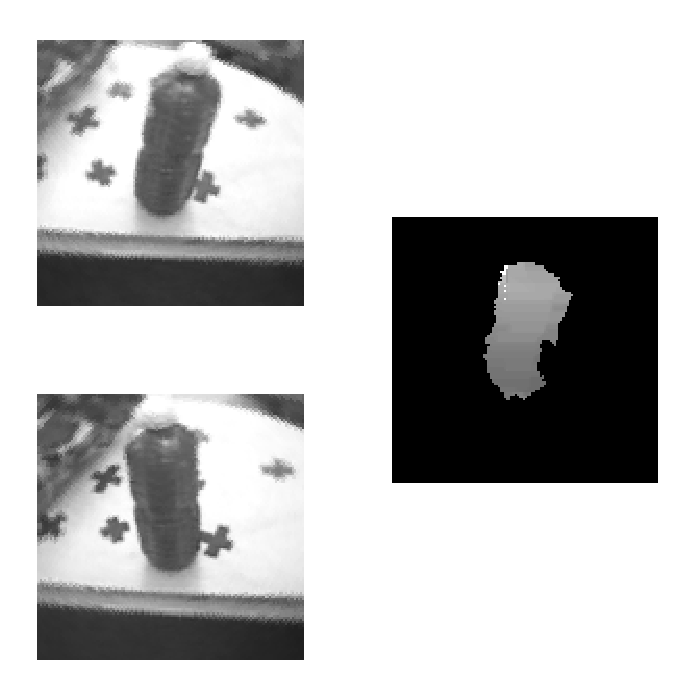
\includegraphics[width=3in]{disparity}
\caption{The Disparity Algorithm  Left: The Stereo Pair, Right: The Final Disparity Map, masked. The mask image comes from the attention algorithm.}
\label{fig-disparity}
\end{figure}

Given a pixel pair $(m,n)$, where $m$ is the $m^{th}$ point on the left scanline and $n$ is the $n^{th}$ point on the right one, each other allowed pair is investigated. The allowance is determined by the monotonicity constraint (a left to right sequence cannot match a right to left sequence on the other image of the pair) and by the constraint that a match sequence cannot contain gaps (the node following $(m,n)$ must contain either $m+1$ or $n+1$).  
Each arc has a cost, which is the sum of the error of the pair (i.e. the difference between the gray values of the two pixels) and a linear error coming from disparity jumps.
\begin{figure}
	\centering
		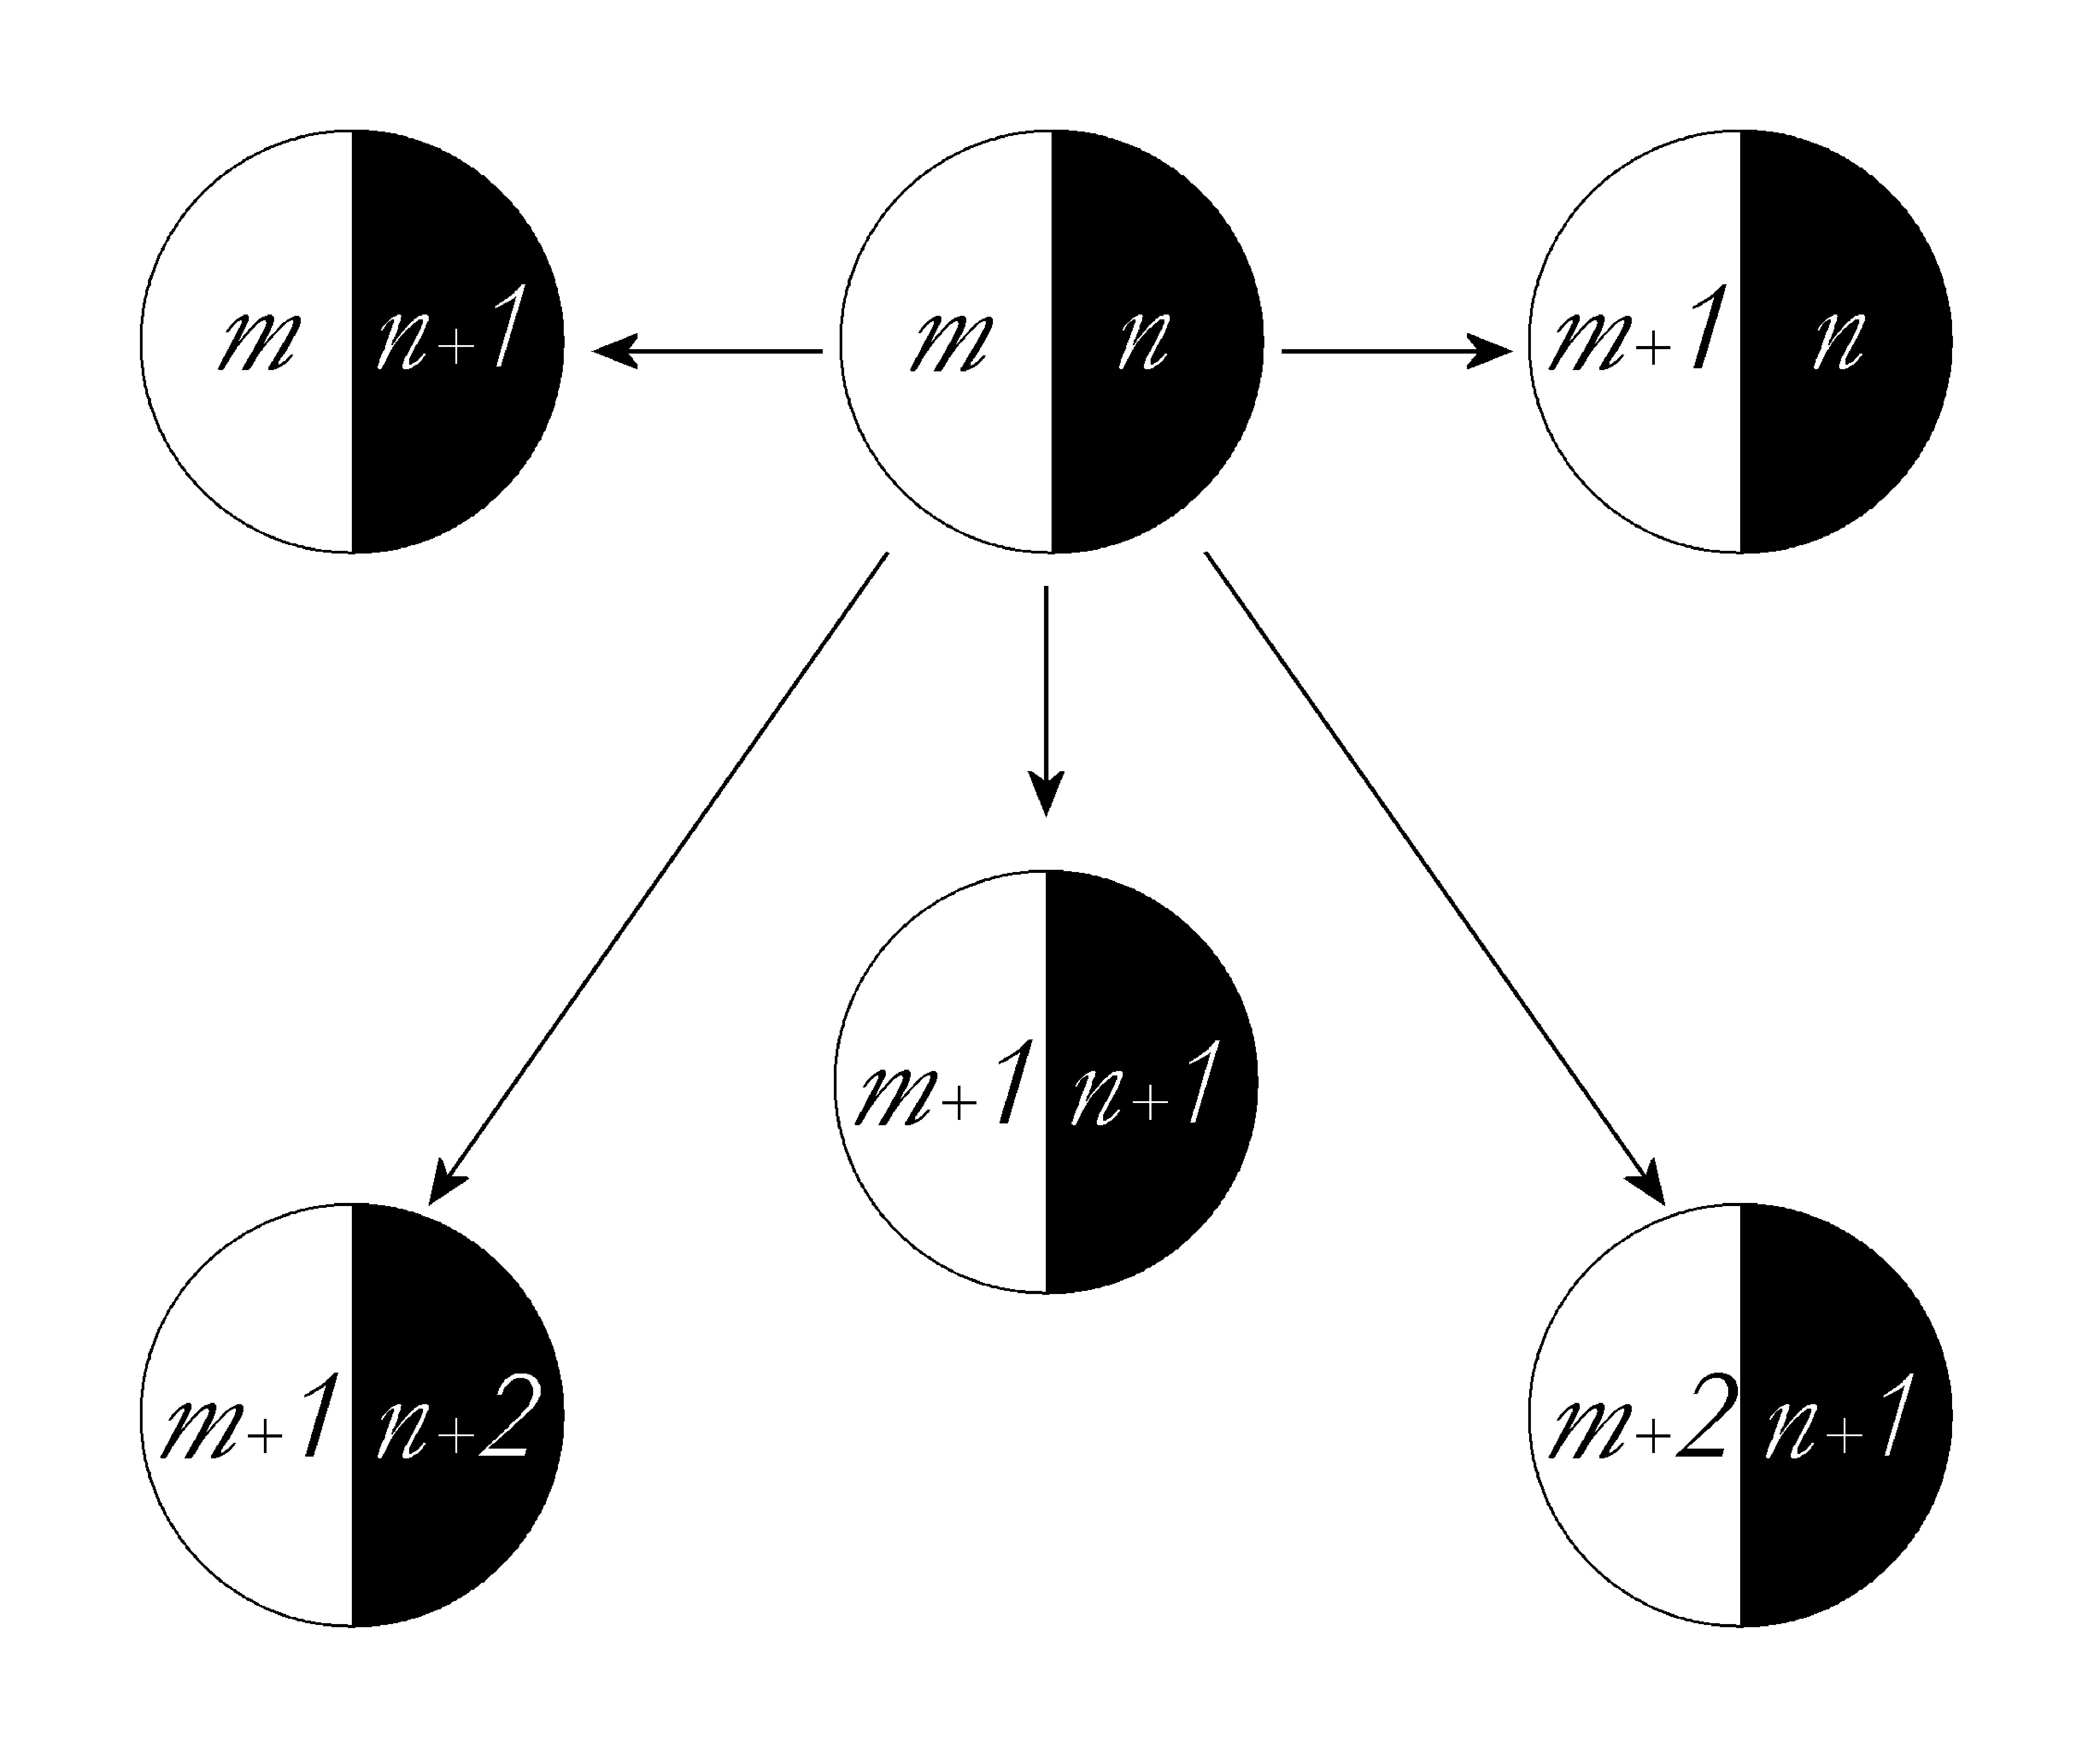
\includegraphics[width=0.70\textwidth]{graph.eps}
	\caption{A section of the graph: the columns have constant disparity $(m-n)$. The upper three nodes show that the uniqueness constraint is not used (a point on one scanline can match more than one point on the other one)}
	\label{fig-graph}
\end{figure}

\section{The Body}
Humans become skillful at controlling their own body after a long period of development and probably thousands of trials. As we discussed in the introduction, however, motor development is extremely important and enable the correct perceptual development of the child. For this reason the robot spends the first phase of its artificial development learning how to correctly control the head and the arm to perform various tasks such as visual tracking and reaching of a target.
Control of the body requires implicit knowledge of its structure (e.g. relative position of the limbs, their size) as well as its dynamical characteristics (e.g. the weight of the body segments). The ensemble of this knowledge is called \emph{body-schema}; experiments in neuroscience have given support to the existence of a body-schema in the primate brain \cite{graziano99whereis,graziano00coding}. Graziano and co-workers have found neurons in the motor of monkeys which code the position of the hand in the visual field.
On the other hand, developmental psychologist have been trying to understand the mechanisms which allow the brain to acquire such representation. As roboticists we are interested in the same mechanisms as they allow the system (biological or artificial) to autonomously acquire and maintain all parameters required to the control of action and avoid manual estimation and calibration. For this reason the problem has been studied by other authors \cite{yoshikawa03doestheinvariance,fitzpatrick04feelthebeat,metta03early}.
We follow here an approach similar to the one of \cite{fitzpatrick04feelthebeat,metta03early} where repeated self-generated actions are exploited for learning. We programmed the robot to perform a period movement of the wrist. This motion is detected by the robot visually and \emph{motorically}. In the former case we Visual motion is computed by image differencing with an adaptive model of the background. In the latter case the robot computes the first derivative of the encoder feedback. The period of motion of each pixel in the motion image is compared to that of the encoders. Pixels whose motion is periodic and whose period matches that of the joints are selected and grouped together to form the segmentation of the hand. Figure ~\ref{fig-handsegmentation} shows an example of the result of this procedure.

\begin{figure}
\centering
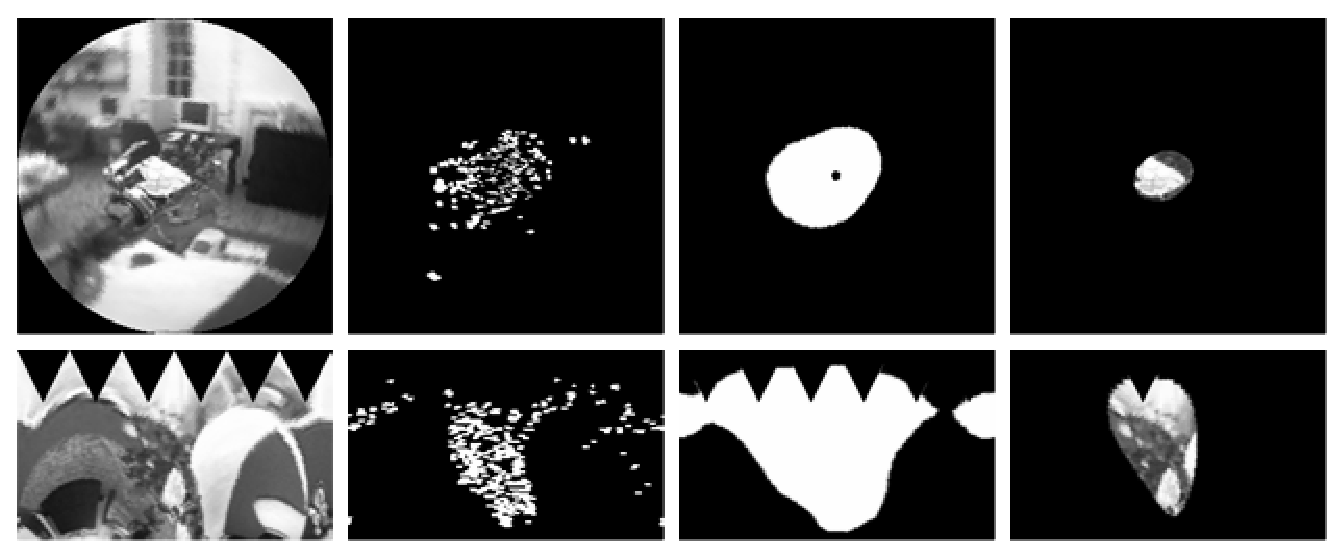
\includegraphics[width=3in]{handsegmentation}
\caption{Hand segmentation: an example.}
\label{fig-handsegmentation}
\end{figure}

We used this procedure to train a neural network to compute of the hand in the visual field given the current robot posture (arm and head joint configuration). Another neural network learns the approximate shape and orientation of the hand given the same information. Figure ~\ref{sec-handlearning1} show the result of this process. 

\begin{figure}
\centering
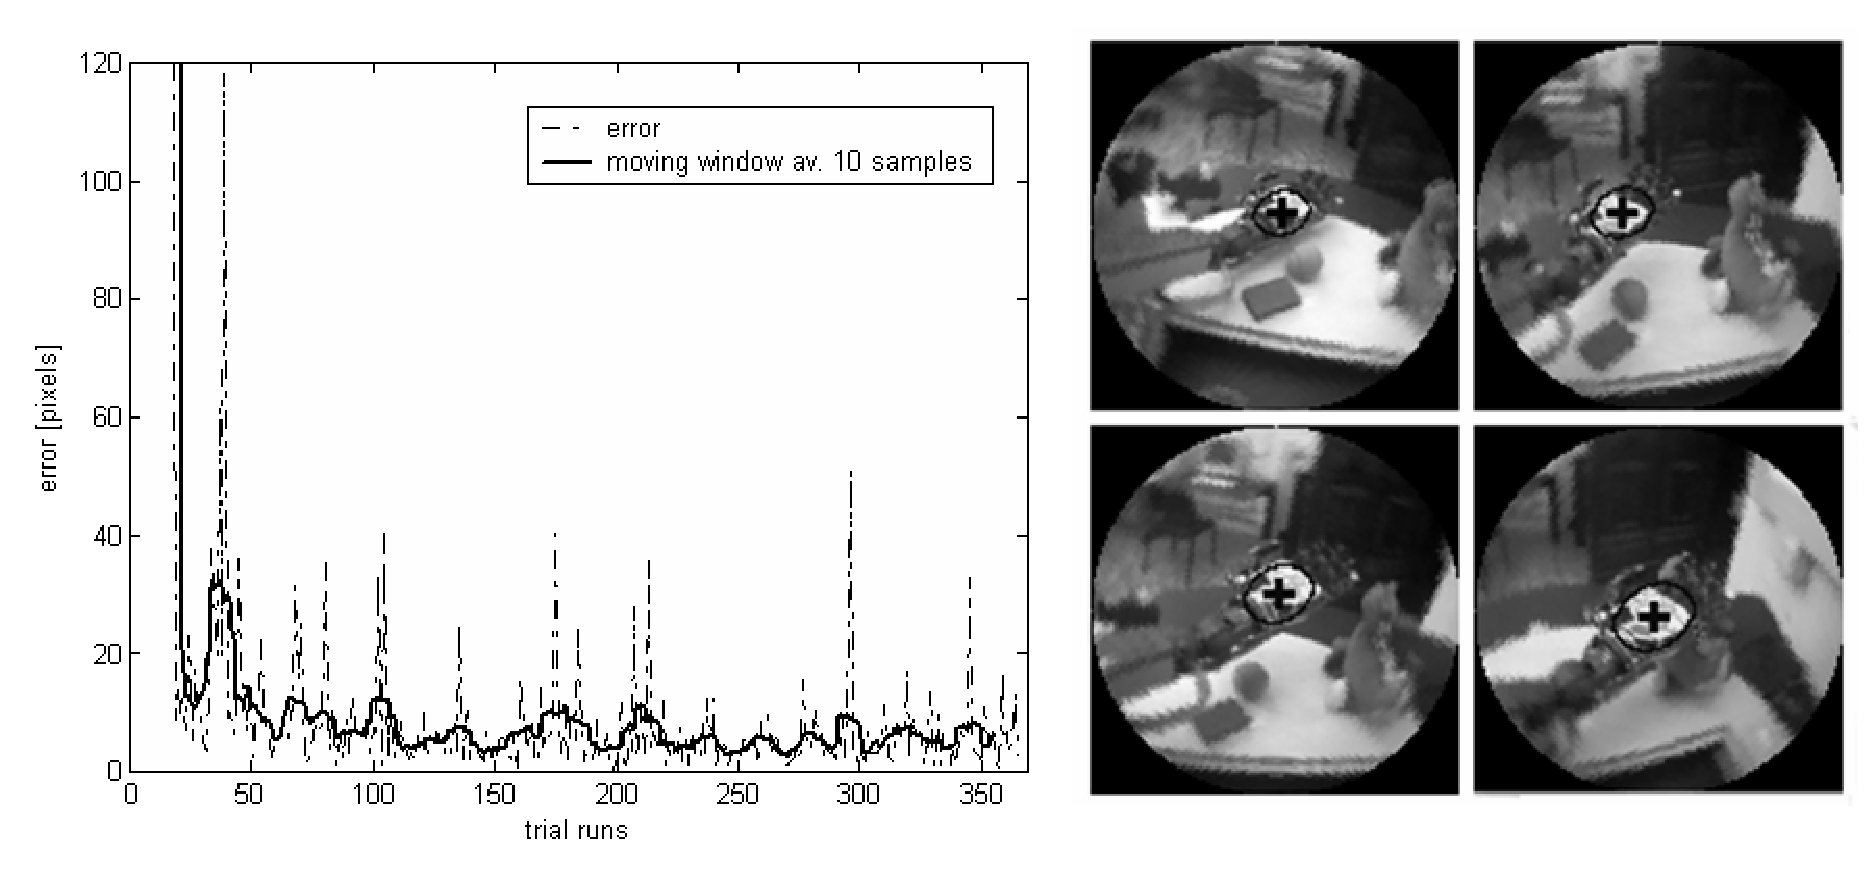
\includegraphics[width=3in]{handlearning1}
\caption{Learning to localize the hand in the visual field.}
\label{sec-handlearning1}
\end{figure}

The role of vision during reaching is still debated \cite{saunders03humans}, although experimental results suggest that sight of the hand is not required for children to start reaching for an object \cite{clifton93isvisually,clifton94multimodal} and is used only relatively late in development to actually adjust the trajectory of the hand during action \cite{ashmead93visual}. 
Sight of the hand, however, might be used to acquire eye-hand coordination. By tracking the hand the robot builds a mapping between each position of the arm and the corresponding head configuration when fixation of the head is achieved. The hypotheses is that reaching starts by first fixating the object; in this condition the fixation point coincides with the target and uniquely identifies its position with respect to the body. The arm motor command can be obtained by a transformation between the head and arm joints, that is by mapping motor variables into motor variables:
\begin{equation}q_{arm}=f(q_{head})\label{motormapping}\end{equation}
where $q_{arm}$ and $q_{head}$ are head and arm posture respectively. This mapping implements the inverse kinematics of the arm and can be easily learnt when the robot looks at its hand. The robot keeps fixation of the hand while moving the arm randomly in the workspace. Every time the arm stops and the eyes have achieved fixation on the hand a new pair arm-head was acquired and used as a training sample to the neural network approximating the mapping of equation \ref{motormapping}. The robot uses the mapping to reach for visually identified objects as soon as a few samples are acquired.
The actual trajectory is computed by linearly interpolating the motor command and the current joint position. The trajectory results in a set of small steps that are effected by a PD controller with gravity compensation. A procedure to learn the gravity load term is explained here \cite{natale04thesis}.

\section{Interaction}
If we had results, we could report them here.
\section{Discussion}
\label{sect:conclusion}
We have shown results on two phases of the acquisition of sensorimotor coordination in a upper body humanoid robot. The system includes a visual attention system employing top-down and bottom-up information. The former is introduced in the system beforehand, whereas the latter is modulated by the robot's interaction with the environment. 

We have shown the importance of the interaction between the environment and the robot for learning. This was demonstrated indirectly, when the robot exploited self-produced actions to explore its own body, and directly when the robot actively explored the visual properties of the objects it grasped.

In the experiment discussed here, we start to link different actions to different objects to investigate the possibility for the robot to autonomously learn what actions are more suitable for different contexts (different objects or environment). Although far from completed, this is meant to enlighten us about the possibility of autonomously enriching the robot's knowledge of the world. This is not only relevant for action, but also from a perceptual point of view. Indeed, actions establish a link between events and the causes that have generated them. In other words by acting in the world an ``active'' agent can link the actions it performs with their consequences. This link can be used in two ways. For planning, to select a particular action required to bring about a desired consequence.

The advantage to use such a representation is that usually goals are more clearly expressed in motoric term, but the only available information when observing somebody else's actions is a perceptual one. I.e. the only information available is the sensorial experience associated with the event. In this case the robot can search its own experience for an event that closely match what it is observing and select the action(s) that generated them. For example the sound of an object that hits the floor can be associated with the action of dropping it. Both problems are interesting and challenging, luckily the solution to both problems appears to be tightly intertwined with sensorimotor development.

It is fair to say that the system developed so far, although complex, still manifest a certain degree of brittleness perhaps associated to the amount of ``handcrafted'' components we were nonetheless forced to use to reach this level of functioning in a reasonable amount of time. For instance the choice of color blobs as features clearly limits the visual system in a way that sometimes prevent the robot from perceiving certain object characteristics. Also, some other times the residual error in reaching goes unnoticed to the robot that eventually fails to grasp the object reliably. On the object recognition side, objects composed of only a few blobs are easily mistaken for other blobs in the background since a single color (or certain blob combinations) is clearly not discriminative enough (the background might present similar combinations). 

We are aware of many of these limitations and, in fact, our ongoing work is exactly aimed at improving the overall performance of the robot both motorically and perceptually with a particular emphasis on the manipulation abilities we deem fundamental for autonomous development.





\section*{Acknowledgments}
This work was supported by European Union grants RobotCub (IST-2004-004370)
and ADAPT (IST-2001-371173).


%  bibliography goes here
\bibliographystyle{./sty/IEEEtran.bst}
\bibliography{main.bib}

\end{document}
